\chapter{Arquitetura EDGAR}
\label{chap:arquitetura}

Este capítulo descreve a arquitetura EDGAR e o funcionamento de seus módulos. A apresentação parte da organização geral e das tecnologias utilizadas, acompanha o processamento dos documentos até a geração de respostas e termina com a interface interativa que permite conferir as evidências no próprio PDF. O ambiente de execução e o protocolo experimental adotados para avaliar a arquitetura são descritos no Capítulo~\ref{chap:metodologia-avaliacao}.

\section{Visão Geral da Arquitetura EDGAR}
\label{sec:visao_geral_arquitetura_edgar}

O EDGAR é uma arquitetura de geração aumentada por recuperação multimodal (MRAG) voltada à consulta de materiais didáticos em PDF. Como esses documentos podem reunir textos, tabelas e figuras em uma mesma página, a arquitetura procura recuperar informações a partir de componentes específicos, sem depender exclusivamente de páginas completas ou de uma sequência linear de texto. Para isso, combina análise visual, extração de conteúdo e recuperação semântica, utilizando modelos previamente treinados, sem treinamento adicional ou ajuste fino (\textit{training-free}).

Seu funcionamento é dividido em dois fluxos complementares. O \textbf{fluxo de ingestão e indexação (\textit{offline})} prepara os documentos, identifica seus componentes e transforma as informações disponíveis em registros que podem ser consultados posteriormente. Com essa preparação concluída, o \textbf{fluxo de recuperação e geração (\textit{online})} utiliza a pergunta do usuário para localizar evidências relevantes e fornecê-las ao modelo responsável pela resposta. A separação permite reutilizar as informações extraídas e descritas durante a ingestão, sem repetir a análise visual do PDF a cada nova pergunta.

A interação com esses fluxos ocorre por meio de uma aplicação \textit{web} desenvolvida em Streamlit, na qual é possível enviar um documento, formular perguntas e examinar as evidências localizadas no próprio PDF. A Figura~\ref{fig:pipeline_edgar} apresenta a organização geral da arquitetura e a relação entre suas etapas de processamento e consulta.

\begin{figure}[H]
\centering
\caption{Visão geral da arquitetura EDGAR: fluxo de ingestão e indexação (\textit{offline}) e fluxo de consulta e geração (\textit{online}).}
\label{fig:pipeline_edgar}
\vspace{0.15cm}
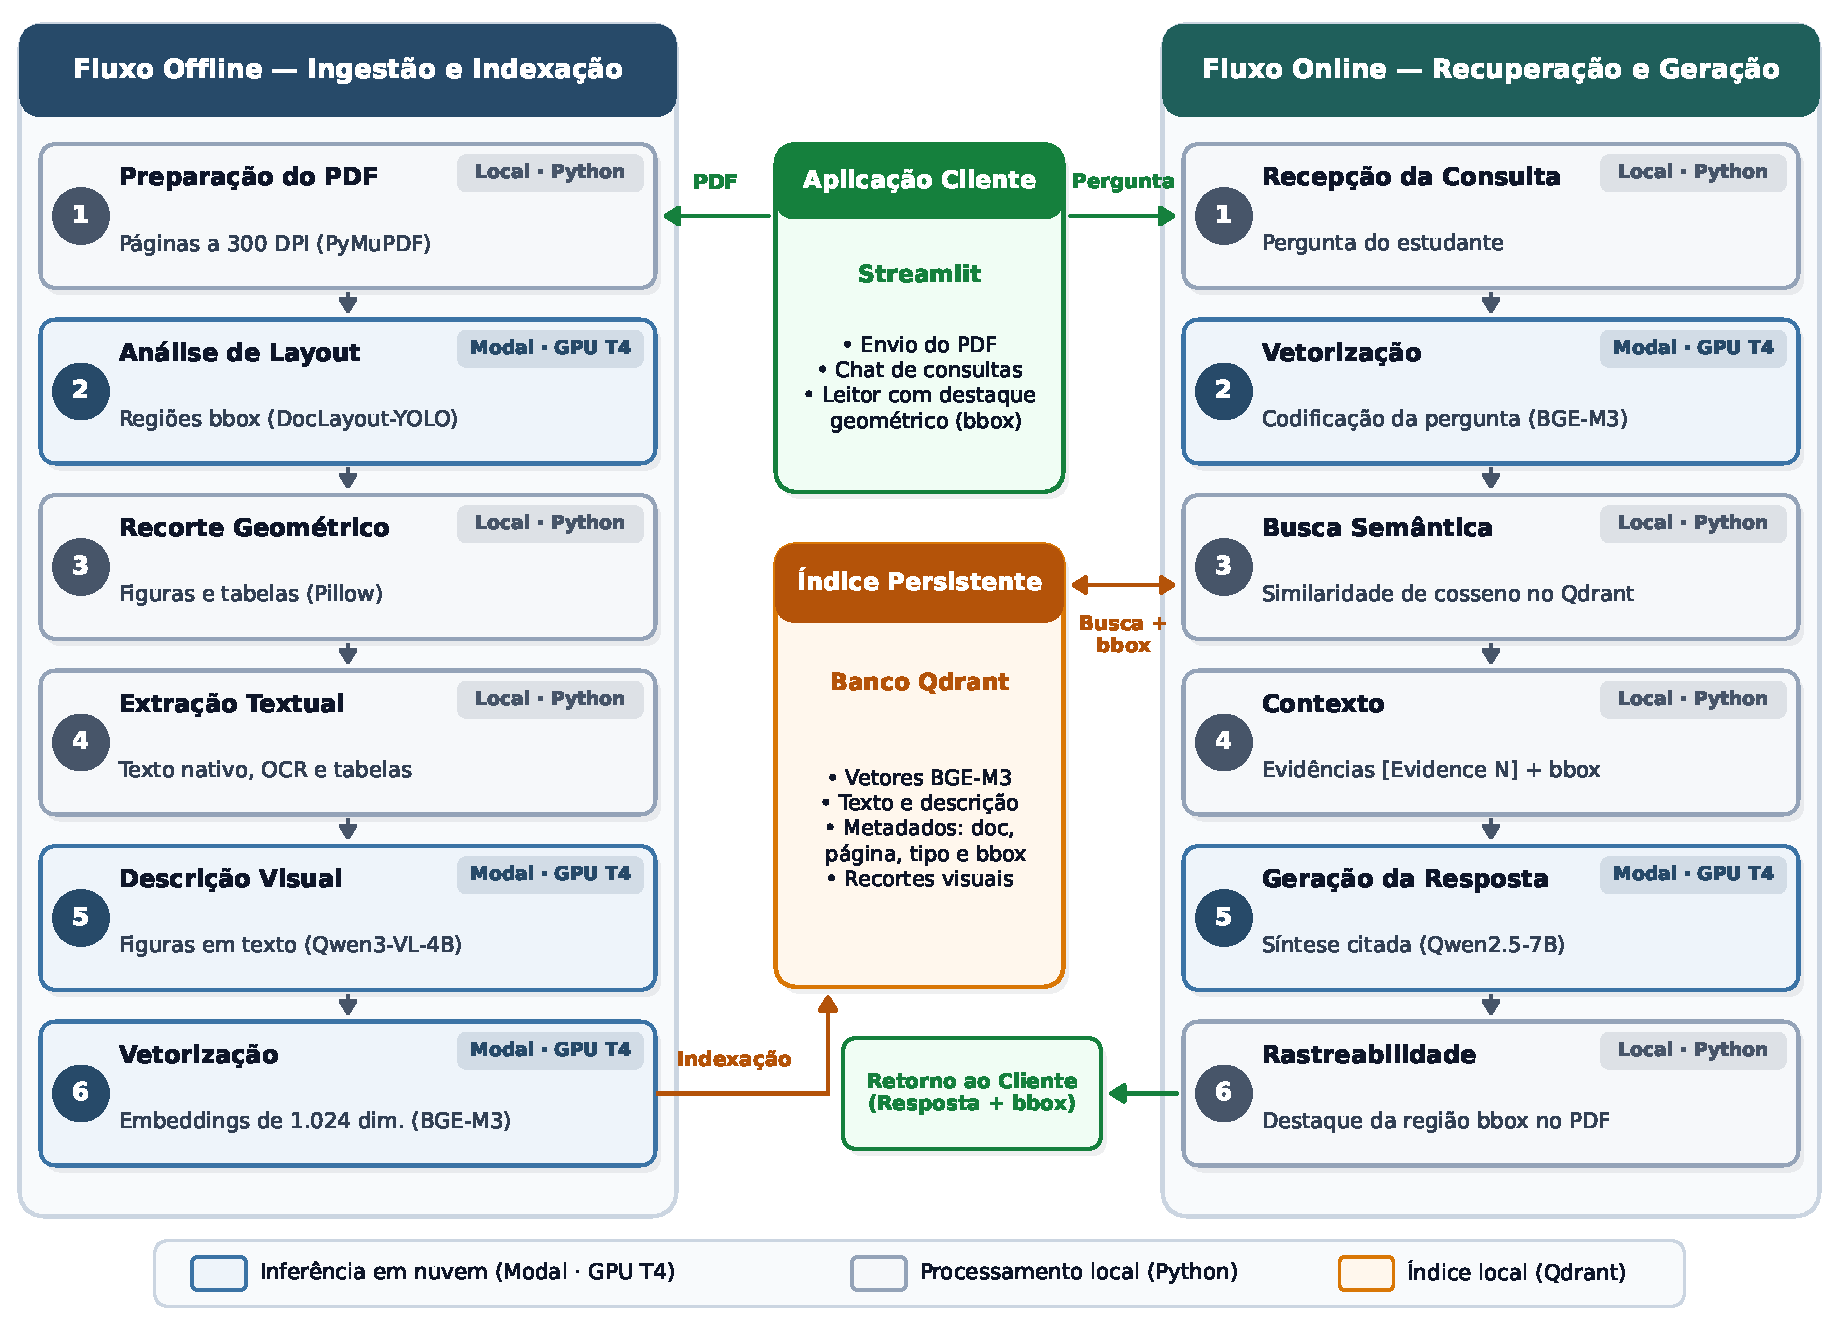
\includegraphics[width=\textwidth]{figuras/pipeline_edgar_modern.pdf}
\vspace{0.05cm}
\legend{Fonte: Elaborado pelo autor.}
\end{figure}

\section{Definição dos Componentes Tecnológicos}
\label{sec:definicao_componentes_tecnologicos}

Para que o conteúdo identificado nas páginas possa ser utilizado nas consultas, o EDGAR reúne ferramentas de processamento de PDFs, análise visual, extração textual e busca vetorial. O Quadro~\ref{quad:componentes-tecnologicos} apresenta as principais tecnologias empregadas e suas funções na arquitetura.

\begin{quadro}[H]
\centering
\caption{Principais componentes tecnológicos utilizados no EDGAR.}
\label{quad:componentes-tecnologicos}
\begingroup
\small
\renewcommand{\arraystretch}{1.18}
\begin{tabularx}{\textwidth}{|p{3.0cm}|p{4.3cm}|X|}
\hline
\textbf{Módulo} & \textbf{Tecnologia} & \textbf{Função} \\
\hline
Preparação de PDFs & PyMuPDF & Renderizar páginas e extrair textos e informações de posicionamento. \\
\hline
Análise de \textit{layout} & DocLayout-YOLO & Identificar componentes e suas coordenadas na página. \\
\hline
Recortes visuais & Pillow (PIL) & Isolar imagens de componentes detectados. \\
\hline
Reconhecimento textual & Tesseract OCR & Recuperar texto quando a extração nativa não produz conteúdo. \\
\hline
Tratamento de tabelas & PyMuPDF e rotinas próprias & Reconstruir, quando possível, cabeçalhos e linhas em formato textual. \\
\hline
Descrição visual & Qwen3-VL-4B-Instruct & Descrever figuras e tabelas sem estrutura textual recuperável. \\
\hline
Representação vetorial & BGE-M3 (Sentence Transformers) & Gerar \textit{embeddings} textuais das evidências e perguntas. \\
\hline
Armazenamento e busca & Qdrant & Indexar vetores e metadados; realizar buscas por similaridade. \\
\hline
Geração de respostas & Qwen2.5-7B-Instruct & Elaborar respostas a partir das evidências recuperadas. \\
\hline
Interface de validação & Streamlit & Receber PDFs e consultas e apresentar respostas e evidências. \\
\hline
\end{tabularx}
\endgroup
\legend{Fonte: Elaborado pelo autor.}
\end{quadro}

As ferramentas atuam em etapas sucessivas e compartilham os metadados necessários para preservar a origem de cada evidência. O PyMuPDF\footnote{\url{https://pymupdf.readthedocs.io}.} e o Pillow\footnote{\url{https://python-pillow.org}.} realizam a leitura dos arquivos PDF e o recorte das regiões visuais, o Qdrant\footnote{Banco de dados vetorial de código aberto: \url{https://qdrant.tech}.} gerencia o armazenamento vetorial e o Streamlit\footnote{Biblioteca Python para criação de aplicações \textit{web}: \url{https://streamlit.io}.} provê a camada de interação com o usuário. Os modelos de visão e linguagem e de representação semântica são abertos e disponibilizados no repositório Hugging Face: Qwen3-VL-4B-Instruct\footnote{\url{https://huggingface.co/Qwen/Qwen3-VL-4B-Instruct}.}, Qwen2.5-7B-Instruct\footnote{\url{https://huggingface.co/Qwen/Qwen2.5-7B-Instruct}.} e BGE-M3\footnote{\url{https://huggingface.co/BAAI/bge-m3}.}.

\section{Fluxo de Ingestão e Indexação}
\label{sec:fluxo_assincrono_ingestao_indexacao}

A ingestão transforma o PDF em um conjunto de registros que poderão ser recuperados durante as consultas. Para isso, o EDGAR identifica as regiões de cada página, extrai ou descreve seu conteúdo e prepara representações textuais para indexação. O fluxo ocorre antes da geração das respostas, de modo que as informações visuais necessárias à busca já estejam disponíveis quando uma pergunta é apresentada.

\subsection{Preparação e segmentação documental}
\label{subsec:fase1_unificacao_visual}
\label{subsec:fase2_analise_layout}
\label{subsec:fase3_isolamento_geometrico}

Para recuperar informações de componentes específicos, o EDGAR precisa primeiro reconhecer como o conteúdo está distribuído nas páginas. O processamento começa com a conversão das páginas do PDF em imagens pelo PyMuPDF, preservando a identificação do documento, o número da página e suas dimensões. Sobre essas imagens atua o modelo DocLayout-YOLO, que localiza elementos como parágrafos, títulos, figuras, tabelas e legendas, produzindo para cada região uma categoria estrutural e suas coordenadas na página.

Essas coordenadas, denominadas \textit{bounding boxes}, delimitam a área ocupada pelos componentes e permitem que suas imagens sejam recortadas com a biblioteca Pillow. Os recortes visuais são gerados para figuras, tabelas e fórmulas isoladas, enquanto a localização dos demais elementos orienta a extração textual localizada. As mesmas coordenadas geométricas permanecem associadas aos componentes para que, após a recuperação, seja possível destacar a região de origem no PDF. A Figura~\ref{fig:dla_exemplo} ilustra o resultado dessa etapa em uma página de livro didático, comparando a página original com as regiões identificadas pelo detector.

\begin{figure}[H]
\centering
\caption{Exemplo de detecção de componentes em uma página do livro \textit{University Physics}.}
\label{fig:dla_exemplo}
\vspace{0.2cm}
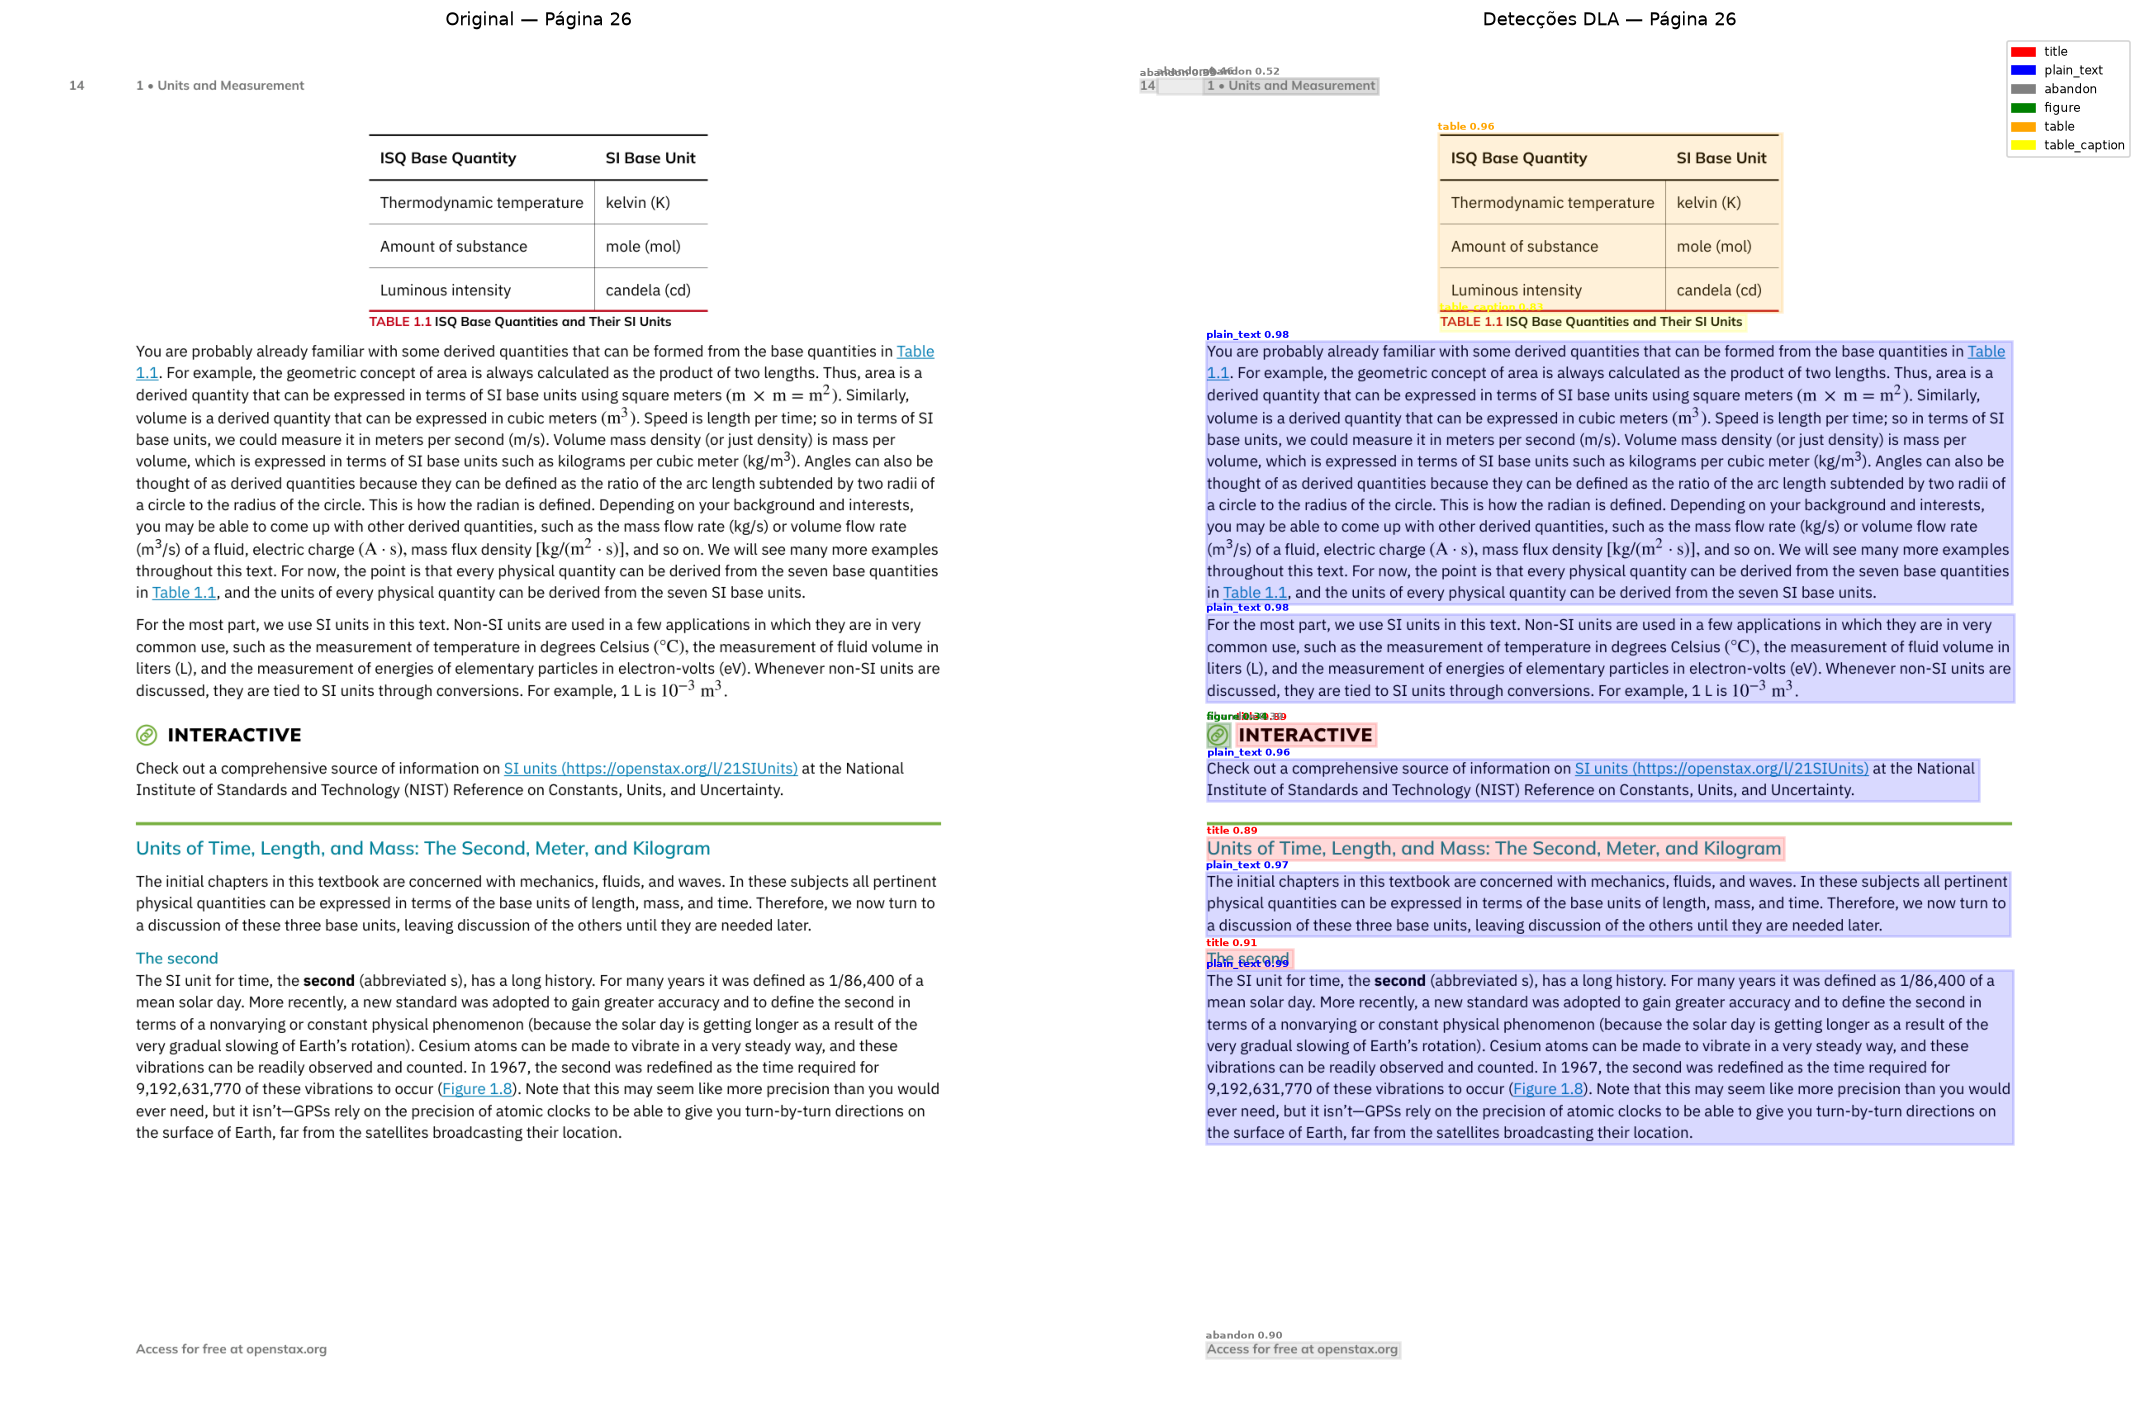
\includegraphics[width=\textwidth]{figuras/dla_pagina26.png}
\legend{Fonte: Elaborado pelo autor, a partir de \citeonline{moebs2016universityphysics}.}
\end{figure}

Na Figura~\ref{fig:dla_exemplo}, os rótulos em inglês correspondem às categorias atribuídas pelo detector a cada caixa delimitadora, acompanhadas do respectivo grau de confiança: \textit{title} (título), \textit{plain\_text} (texto corrido), \textit{table} (tabela), \textit{table\_caption} (legenda de tabela), \textit{figure} (figura) e \textit{abandon} (elementos periféricos como cabeçalhos e rodapés, que são descartados antes da indexação).

\subsection{Extração textual e descrição visual}
\label{subsec:fase4_ocr_localizado}
\label{subsec:fase5_descricao_visual}

Uma vez identificadas as regiões da página, o tratamento do conteúdo varia conforme as informações disponíveis em cada componente. Nos elementos textuais, o EDGAR procura primeiro o texto existente no próprio PDF, utilizando o PyMuPDF e as coordenadas da região detectada. Quando essa extração não retorna conteúdo, o Tesseract OCR é aplicado à área correspondente. Assim, o reconhecimento por OCR funciona como alternativa para regiões sem texto digital acessível, em vez de ser executado indiscriminadamente em todas as páginas.

As tabelas exigem um tratamento adicional porque a simples extração de palavras pode não conservar a relação entre cabeçalhos e valores. Por esse motivo, o sistema tenta reconstruir sua organização a partir da posição dos textos, formando uma representação de linhas e colunas quando há informações suficientes. Se essa reconstrução não for possível, a imagem da tabela é encaminhada para descrição visual.

Nas figuras, cuja informação muitas vezes depende de relações gráficas que não aparecem como texto extraível, o modelo Qwen3-VL-4B-Instruct produz descrições em linguagem natural a partir dos recortes. O mesmo modelo é utilizado nas tabelas que não possuem estrutura textual recuperável. Essas descrições permitem incorporar à busca informações originalmente apresentadas de forma visual, mas representadas em texto antes da indexação.

\subsection{Representação e indexação das evidências}
\label{subsec:fase6_indexacao_hibrida}

O conteúdo obtido nas etapas anteriores é organizado em uma representação textual para cada componente indexável. Em parágrafos e títulos, essa representação provém do texto extraído. Nas figuras, utiliza-se a descrição visual, acompanhada de informações textuais associadas quando disponíveis; nas tabelas, emprega-se a estrutura reconstruída ou, na ausência desta, a descrição produzida pelo modelo visual. A preparação incorpora ainda textos de legendas e notas quando esses elementos estão vinculados ao componente correspondente.

A partir dessas representações, o modelo BGE-M3 gera \textit{embeddings} textuais densos, que são armazenados no Qdrant junto aos metadados de cada registro: identificador do componente, documento de origem, página, tipo estrutural, coordenadas geométricas (\textit{bbox}), texto ou descrição e referência ao recorte visual. Para ilustrar essa estrutura, o Código-fonte~\ref{lst:registro} apresenta, de forma simplificada, um registro JSON armazenado no índice.

\noindent\begin{minipage}{\textwidth}
\begin{lstlisting}[language=json,basicstyle=\ttfamily\footnotesize,frame=single,aboveskip=0.25cm,belowskip=0.10cm,caption={Exemplo simplificado de um registro JSON indexado no Qdrant.},label={lst:registro}]
{
  "component_id": "e40d6bf9-9076-5cac-8110-...",
  "document": "physics_001.pdf",
  "page": 77,
  "component_type": "table",
  "bbox": {"x1": 299, "y1": 234, "x2": 2249, "y2": 886},
  "text": "Table caption: TABLE 4.1 Typical
           Centripetal Accelerations
           Columns: Object | Centripetal
           Acceleration (m/s2 or factors of g) ...",
  "vector": [0.012, -0.034, ..., 0.027]
}
\end{lstlisting}
\noindent{\normalsize Fonte: Elaborado pelo autor.}
\end{minipage}\vspace{0.35cm}

No Código-fonte~\ref{lst:registro}, o campo \texttt{bbox} guarda as coordenadas do retângulo que delimita o componente na página renderizada, o campo \texttt{text} reúne a representação textual indexada (neste caso, a legenda e as colunas reconstruídas da tabela) e o campo \texttt{vector} armazena o \textit{embedding} numérico utilizado na busca por similaridade de cosseno. Desse modo, a representação empregada para localizar uma evidência permanece vinculada à sua posição exata no material original.

\section{Fluxo de Recuperação e Geração}
\label{sec:fluxo_sincrono_recuperacao_geracao}

Com os documentos previamente indexados, o EDGAR atende às consultas utilizando as representações já preparadas. Nesse fluxo, a pergunta do usuário orienta a busca por evidências e a montagem do contexto fornecido ao modelo gerador, mantendo a inferência visual separada do momento da resposta.

\subsection{Recuperação semântica das evidências}
\label{subsec:fase7_recuperacao_evidencias}

A recuperação começa quando a pergunta é convertida em um vetor pelo mesmo modelo BGE-M3 utilizado na indexação. O Qdrant compara esse vetor aos registros armazenados por meio da similaridade de cosseno e retorna os componentes mais próximos, acompanhados de suas representações textuais e metadados de origem. Na aplicação interativa, a busca pode ser filtrada para consultar apenas o documento ativo enviado pelo usuário.

\subsection{Organização do contexto e geração de respostas}
\label{subsec:fase8_engenharia_contexto}

Os componentes recuperados são reunidos em um contexto textual estruturado conforme a ordem de relevância da busca. Cada evidência recebe um identificador sequencial e é acompanhada de seus metadados de página, tipo de componente e localização. Esse contexto é enviado ao modelo Qwen2.5-7B-Instruct junto à pergunta do usuário e às instruções para fundamentar a resposta exclusivamente nas fontes fornecidas, citando as evidências utilizadas.

Durante a geração, o modelo recebe as representações textuais construídas na ingestão (textos extraídos, tabelas reconstruídas e descrições visuais), mantendo a busca e a geração apoiadas no mesmo conteúdo indexado. Após a inferência, a resposta gerada é retornada junto à lista de evidências e seus metadados geométricos para exibição ao usuário.

\section{Interface Interativa de Validação}
\label{sec:interface_validacao}
\label{subsec:interacao_aplicacao_cliente}

A aplicação desenvolvida em Streamlit reúne a consulta ao EDGAR e a visualização do documento em uma única interface. O usuário pode enviar um PDF, acompanhar seu processamento e fazer perguntas em linguagem natural sem precisar operar diretamente os módulos internos da arquitetura.

Além de apresentar as respostas em uma área de conversa, a interface mantém um leitor de PDF integrado para inspeção das fontes citadas. Quando o usuário seleciona uma evidência retornada, a aplicação navega até a página correspondente e desenha uma marcação visual sobre a região delimitada pelas coordenadas (\textit{bbox}) armazenadas, permitindo verificar diretamente no documento original o componente que fundamentou a resposta.
